\begin{frame}{Software architecture}

    \tikzstyle{mainblock} = [rectangle, rounded corners, minimum width=3cm, minimum height=2cm,text centered, draw=black, fill=red!30]
    \tikzstyle{arrow} = [thick,->,>=stealth]
    \vspace{0.2cm}
    \centering
    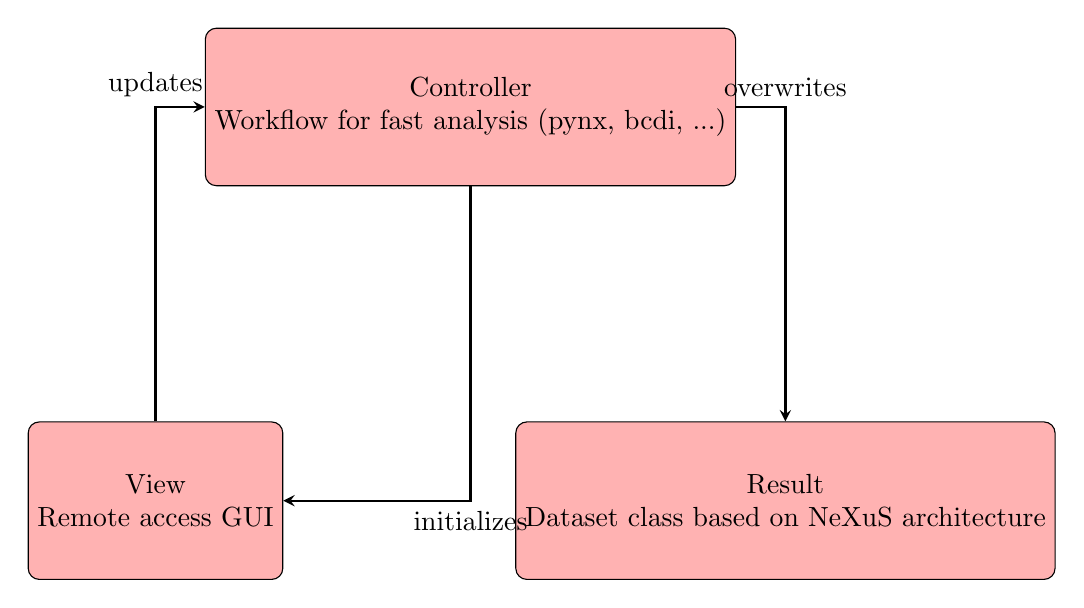
\begin{tikzpicture}[node distance=4cm]
        \node (controller) [mainblock, align=center] {Controller\\Workflow for fast analysis (pynx, bcdi, ...)};
        \node (result) [mainblock, right of=controller, yshift=-5cm, align=center] {Result\\Dataset class based on NeXuS architecture};
        %\node (logo) [right of=controller, xshift=2cm, yshift=1cm] {\includegraphics[width=.1\textwidth]{Figures/logo/pythonlogo.png}};
        
        \node (view) [mainblock, left of=controller, yshift=-5cm, align=center] {View\\Remote access GUI};
        
        \draw [arrow] (controller) |- node[anchor=north] {initializes} (view);
        \draw [arrow] [above] (view) |- node[anchor=south] {updates} (controller);
        \draw [arrow] [right] (controller) -| node[anchor=south] {overwrites} (result);
    \end{tikzpicture}
    
\end{frame}